\subsection{REpresentational State Transfer (REST)}
\label{standard:rest}

En el capítulo 5 de su tesis doctoral, Roy Fielding define el estilo de arquitectura de las aplicaciones web o, en términos más generales, de los sistemas distribuidos basados en hypermedia. Esta arquitectura, a la que denomina \gls{acro:rest}, está presentada como una derivación a partir de las restricciones de interacción que impone, partiendo de un estilo base sin restricciones, al que va agregando otras limitaciones hasta llegar a definir el modelo \gls{acro:rest}. Al realizar la caracterización de esta forma, Fielding logra de forma natural analizar qué propiedades surgen a partir de cada restricción aplicada.

En esta sección desarrollaremos sintéticamente los elementos de \gls{acro:rest} de manera tal que podamos utilizarlos como marco teórico en el desarrollo de nuestra propuesta para la nueva nube de servicios de la \unlp, complementando lo que se ha expuesto en la \autoref{soa:definicion}.


\subsubsection{Derivación de REST}
\label{standard:rest:derivacion}

En este apartado resumiremos el proceso de derivación que realiza Fielding para, a partir de un estilo base al que se le van agregando restricciones o propiedades, llegar a definir el estilo de aplicaciones distribuidas \gls{acro:rest}.

\paragraph{Estilo base}

La derivación de \gls{acro:rest} parte de un estilo de sistemas distribuidos base en el que no existen restricciones ni límites entre los elementos que lo componen.


\paragraph{Cliente-Servidor}

Las primeras restricciones aplicadas al estilo base son aquellas del estilo Cliente-Servidor\cite[Sec.~3.4.1]{tesis:fielding}, en el que un componente Servidor ofrece un conjunto de servicios y escucha peticiones a los mismos, mientras que un componente Cliente realiza solicitudes indicando que desea se realicen esos servicios a través de un \textit{conector}. Ante la recepción de la petición, el Servidor rechaza o realiza lo solicitado y envía en retorno una respuesta al Cliente.
Estas adiciones al conjunto, inicialmente vacío, de limitaciones beneficia al principio de separación de responsabilidades y permite que los componentes Cliente y Servidor evolucionen independientemente, habilitando a una gran escalabilidad de esta arquitectura.


\paragraph{Sin estado}

Tomando ahora como base el estilo Cliente-Servidor, se agrega la restricción de que el Servidor no puede contener información del estado de la sesión\cite[Sec.~3.4.3]{tesis:fielding}: las peticiones realizadas al Servidor deben incluir toda la información necesaria para reflejar el estado actual de la comunicación.

De esta forma, se obtienen nuevas propiedades positivas para el estilo en evolución: visibilidad, confiabilidad y escalabilidad. El sistema gana en visibilidad ya que dado un requerimiento, no se necesita ningún dato adicional para conocer su naturaleza; es más confiable ya que recuperarse, al menos en forma parcial, de un fallo implica simplemente retomar el requerimiento que falló; y la falta de información de estado del lado del Servidor, simplifica su implementación y permite escalar fácilmente instancias del servidor que puedan atender esos requerimientos. Como contrapunto, este conjunto de restricciones tiende a ser penalizado con una performance disminuida sobre las comunicaciones de red, al necesitar incluir y repetir la información del estado en cada petición.


\paragraph{Cache}

A fin de disminuir las penalidades en performance que trae aparejadas el modelo Sin estado definido en el apartado anterior mejorando la eficiencia en el uso de la red, se agrega la restricción del uso de Cache de respuestas\cite[Sec.3.4.4]{tesis:fielding}. La Cache funciona como intermediario entre el Cliente y el Servidor, encargándose de almacenar las respuestas \textit{marcadas como cacheables} por el Servidor de manera tal que peticiones posteriores equivalentes a una anterior con estas características puedan obtener la misma respuesta sin llegar a consultar al Servidor.

Esta adición puede eliminar parcial o inclusive completamente algunas interacciones entre Cliente y Servidor, mejorando la eficiencia de uso de recursos de red y la performance perceptible desde el punto de vista del usuario.

Si bien este punto de la tesis de Fielding hace referencia a la Cache únicamente del lado del Cliente, nosotros tomaremos una postura más general, en la que la Cache puede ubicarse tanto del lado del Cliente como del Servidor, para poder incluir en este estilo a las Cache compartidas o Cache de \eng{Gateway}. Éste tipo de caches funcionan más cercanas al Servidor y permiten que, sin importar si los clientes implementan mecanismos de caching de respuestas, se reduzca la cantidad de requerimientos que efectivamente llegan a ser procesadas por el Servidor, al cachear las respuestas marcadas como cacheables e interceptar las peticiones que los clientes realizan, respondiendo con las respuestas cacheadas que dispongan en caso de aplicar. Las caches de Gateway también permiten alivianar la carga del Servidor cuando múltiples clientes realizan peticiones repetitivas.

El posible problema de agregar la Cache al estilo de arquitectura anterior es que existe la posibilidad de que un recurso cacheado esté desactualizado (\eng{stale}, como se lo referencia comúnmente en inglés) con respecto a la respuesta que el Servidor proveería si esa petición le llegase.


\paragraph{Interfaz uniforme}

Uno de los puntos centrales que aporta \gls{acro:rest} en su definición es la importancia que da a la necesidad de una interfaz uniforme entre los componentes de la arquitectura. Mediante la generalización del diseño del conector utilizado en las comunicaciones y la forma en que se transfiere la información, se simplifica la arquitectura general, a costo de no hacer el uso más eficiente posible de la forma de transmitir los datos, al hacerlo de una forma estandarizada y no una hecha a medida acorde a la información que se necesita intercambiar. La interfaz normalizada que \gls{acro:rest} define está pensada para lograr eficiencia al transferir datos \gls{term:hypermedia} - como es el caso de la web - pero puede resultar subóptima para otro tipo de interacciones. La forma de lograr esta uniformidad es a partir de restricciones: un mecanismo unívoco para la identificación de recursos, la manipulación de estos recursos mediante representaciones, el uso de mensajes autodescriptivos y, principalmente, \gls{acro:hateoas}: el uso de \gls{term:hypermedia} como el motor del estado de la aplicación.


\paragraph{Sistema en capas}

La siguiente limitación que agrega la derivación en la que Fielding define \gls{acro:rest} es la de un sistema desarrollado en capas. Este estilo permite que la arquitectura se componga de capas jerárquicas que se conectan unas a otras de forma tal que un componente no pueda tener conocimiento más allá de la capa con la que está interactuando. Esta forma de concebir las interacciones permite que las capas abstraigan de la complejidad y la posible heterogeneidad de los sistemas que ocultan, y que se uso simplifique la escalabilidad de los sistemas al poder agregar capas que funcionen como balanceadores de carga.


\paragraph{Código bajo demanda}

Por último, se agrega la restricción que identifica la forma de comunicación de la web: los Clientes son entidades con una funcionalidad general, capaces de interpretar el código que el Servidor le envía como respuesta a sus peticiones, a partir del cual obtienen el conocimiento específico. La forma en que se transmite este \eng{know-how} al Cliente es mediante \eng{scripts}\footnote{En su especificación, Fielding además incluye los applets como medios, pero los obviaremos por tratarse de una tecnología en desuso en la actualdad, reemplazada y superada ampliamente por JavaScript.} que extienden esa funcionalidad básica, beneficiando a la extensibilidad del sistema general, pero reduciendo la visibilidad, por lo cual esta restricción es opcional.


\subsubsection{Elementos de la arquitectura REST}
\label{standard:rest:elementos}

\paragraph{Elementos de datos}

\gls{acro:rest} basa las interacciones (la transmisión de la información) en el conocimiento compartido de los tipos de datos a través de la inclusión de metadatos. Los componentes se comunican transfiriendo los recursos utilizando formatos de representación estandarizados, elegidos acorde a lo solicitado por el receptor y la naturaleza del recurso. De esta forma, la información se compone de los siguientes elementos de datos:

\begin{itemize}
  \item \textbf{Recursos e identificadores de recursos:} los recursos son la principal abstracción de \gls{acro:rest}, y hacen referencia a un conjunto de propiedades de una entidad en un momento dado del tiempo. Esas propiedades pueden ser representaciones de recursos o identificadores de recursos, cuya semántica es lo que efectivamente diferencia un recurso de otro. \gls{acro:rest} utiliza los identificadores de recursos en la forma en que la web utiliza \glspl{acro:url} y \glspl{acro:urn} para referenciar recursos utilizando \gls{term:hypermedia}.

  \item \textbf{Representaciones:} los componentes las utilizan para operar sobre el estado actual de un recurso y transmitirla entre sí. Una representación consiste de datos, metadatos para describirlos y, en algunos casos, metadatos para describir a los anteriores (también llamados datos de control), por ejemplo para validar la integridad de un mensaje. Los metadatos tienen la forma clave-valor, donde las claves obedecen al estándar que define la estructura y semántica del valor. La forma de describir la estructura de la información se llama \eng{media type}.
\end{itemize}


\paragraph{Conectores}

El estilo de arquitectura \gls{acro:rest} utiliza diferentes tipos de conectores para encapsular el acceso a los recursos y la transferencia de sus representaciones. Estos tipos se agrupan en:

\begin{itemize}
  \item \textbf{Clientes:} junto a los servidores, son el tipo principal de conectores. Inician las comunicaciones al enviar una solicitud a un servidor.

  \item \textbf{Servidores:} esperan recibir (``escuchan'') solicitudes (``conexiones'') de los clientes, a las que responden a fin de dar acceso a sus servicios.

  \item \textbf{Caches:} pueden encontrarse en conexión a un cliente o un servidor. Su función es almacenar respuestas marcadas como cacheables para evitar realizar subsiguientes peticiones similares.

  \item \textbf{Resolvers:} traducen identificadores de recursos a la información efectiva de red necesaria para conectar los distintos componentes involucrados.

  \item \textbf{Túneles:} permiten realizar conexiones entre componentes que crucen alguno de los límites impuestos por la arquitectura en capas, generando comunicaciones directas entre componentes que de otra forma no podrían tener contacto.
\end{itemize}

Los conectores tienen una interfaz abstracta para establecer las comunicaciones entre los componentes, lo cual oculta los detalles del funcionamiento de conexión interno, separa las responsabilidades y permite que la implementación de cualquier parte del sistema sea remplazada sin afectar al resto de las entidades involucradas. En su funcionamiento, utilizan dos conjuntos de elementos en los mensajes, uno para el de la solicitud y otro para el de la respuesta. El primero consiste en datos de control de la solicitud (por ejemplo, para definir el formato en que se desea el recurso), un identificador de recurso (para indicar a qué recurso se desea acceder), y una representación opcional (por ejemplo, los datos con los que se quiere actualizar una entidad). El conjunto de elementos utilizado en las respuestas se compone de datos de control para la respuesta (como información necesaria para alojar la respuesta en una cache), opcionalmente metadatos del recurso (como \eng{links} relacionados al recurso), y una representación (por ejemplo, el recurso solicitado en sí), también opcional.


\paragraph{Componentes}

Las partes que conforman la arquitectura de los sistemas \gls{acro:rest} se pueden clasificar acorde a su rol en las interacciones en:

\begin{itemize}
  \item \textbf{\eng{User agent}:} utiliza un conector cliente para enviar una solicitud, iniciando una comunicación, y luego espera una respuesta, la cual al llegar finalizará la interacción.

  \item \textbf{\eng{Proxy}:} componente intermediario que funciona más cercano al lado del cliente, encapsulando la interfaz hacia otros servicios y, opcionalmente, brindando otras funcionalidades como traducción de información, mejoras de performance y medidas adicionales de seguridad. Funciona con conectores cliente y servidor para transmitir los mensajes (solicitudes y respuestas) que llegan a él.

  \item \textbf{\eng{Gateway} o \eng{Reverse proxy}:} otro componente intermediario, este más cercano al servidor de origen, también encapsula servicios y puede brindar traducción de los datos que por él circulan, optimizaciones en la performance y realizar acciones para mitigar posibles problemas de seguridad. Al igual que un \eng{proxy}, funciona como cliente y servidor a la vez, reenviando la información que por él pase.

  \item \textbf{Servidor de origen:} utiliza un conector de servidor para recibir solicitudes dirigidas a sus recursos. Las peticiones que le llegan obedecen a una estructura jerárquica que define cómo acceder a los servicios que provee.
\end{itemize}


\subsubsection{REST aplicado a nuestro trabajo}
\label{standard:rest:aplicado}

\todo{Relacionar REST con nuestra propuesta}
\textbf{\textit{@ncuesta: Estaría bueno cerrar este tema con un breve análisis de cómo REST se aplica a nuestro trabajo, para dar un ejemplo concreto de todo lo definido antes. Utilizar como referencia el capítulo 6 de Fielding: https://www.ics.uci.edu/~fielding/pubs/dissertation/evaluation.htm}}

\begin{figure}
  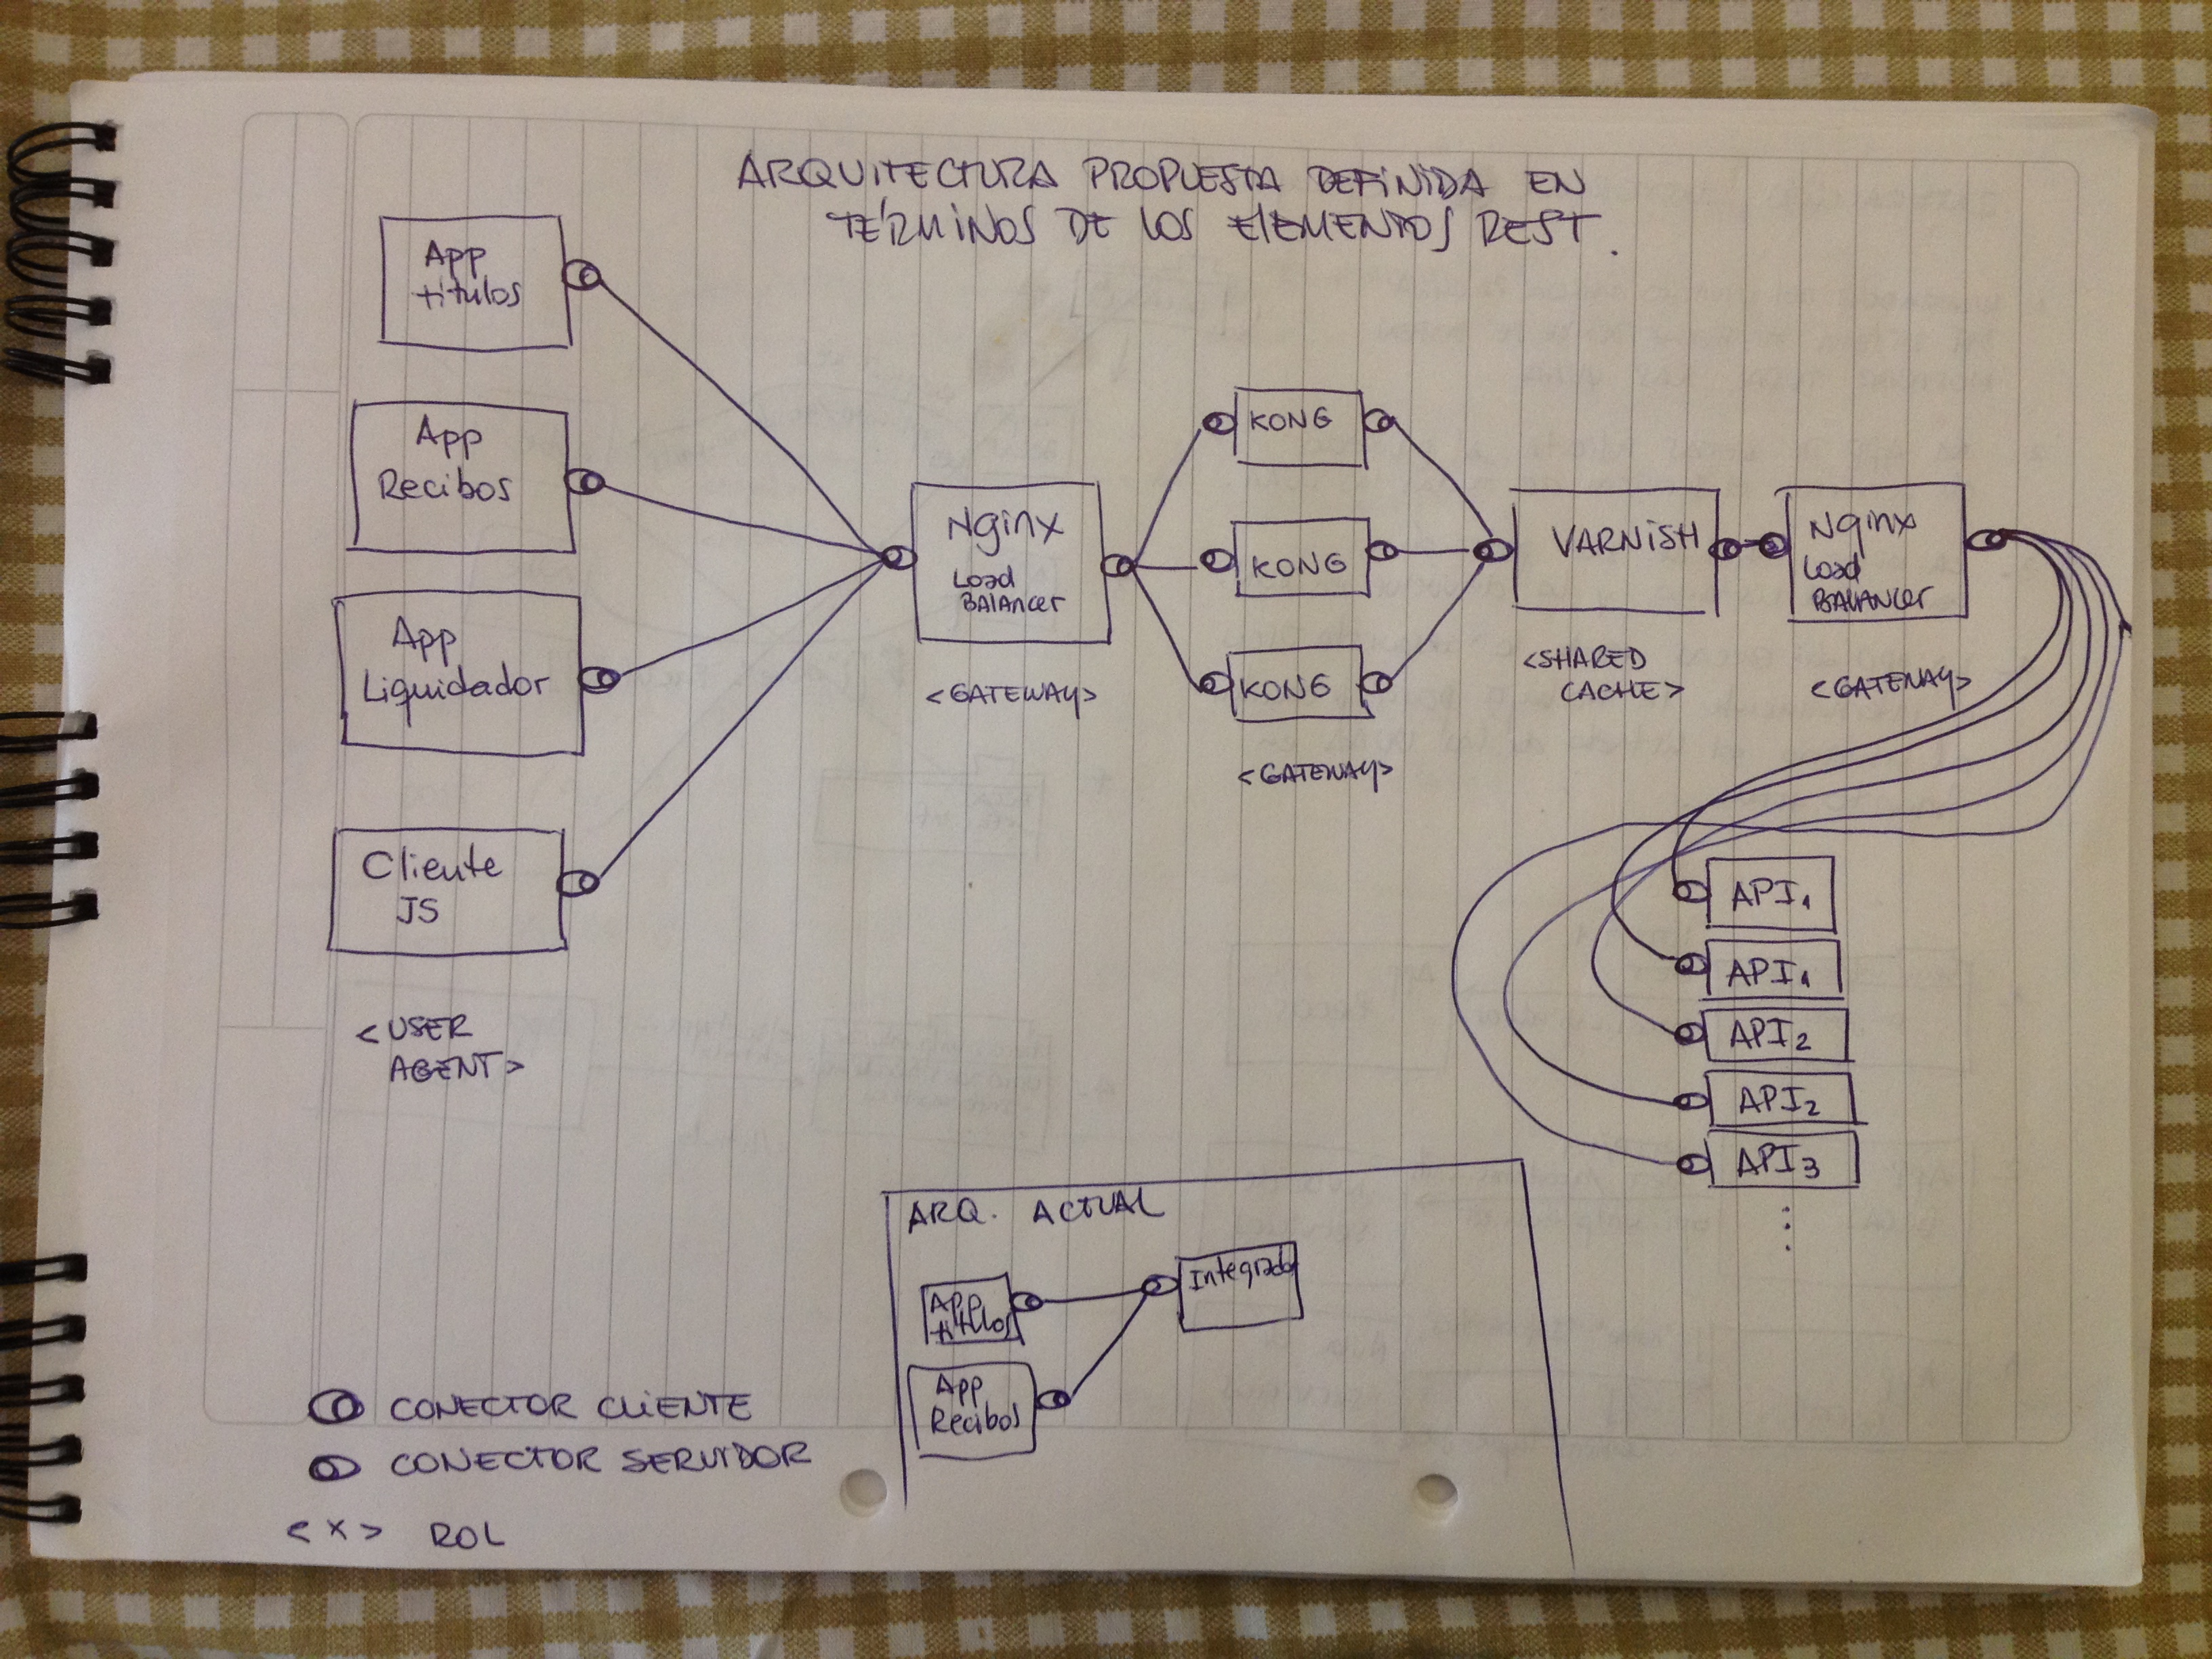
\includegraphics[width=\linewidth]{src/images/sin-organizar/nueva-arq-segun-rest.jpg}
  \caption{Visión \gls{acro:rest} de la nueva arquitectura propuesta}
  \label{fig:ejemplo-rest-nueva-arquitectura}
\end{figure}
